\documentclass{standalone}
\usepackage{tikz}
\usetikzlibrary{patterns, positioning}


\begin{document}
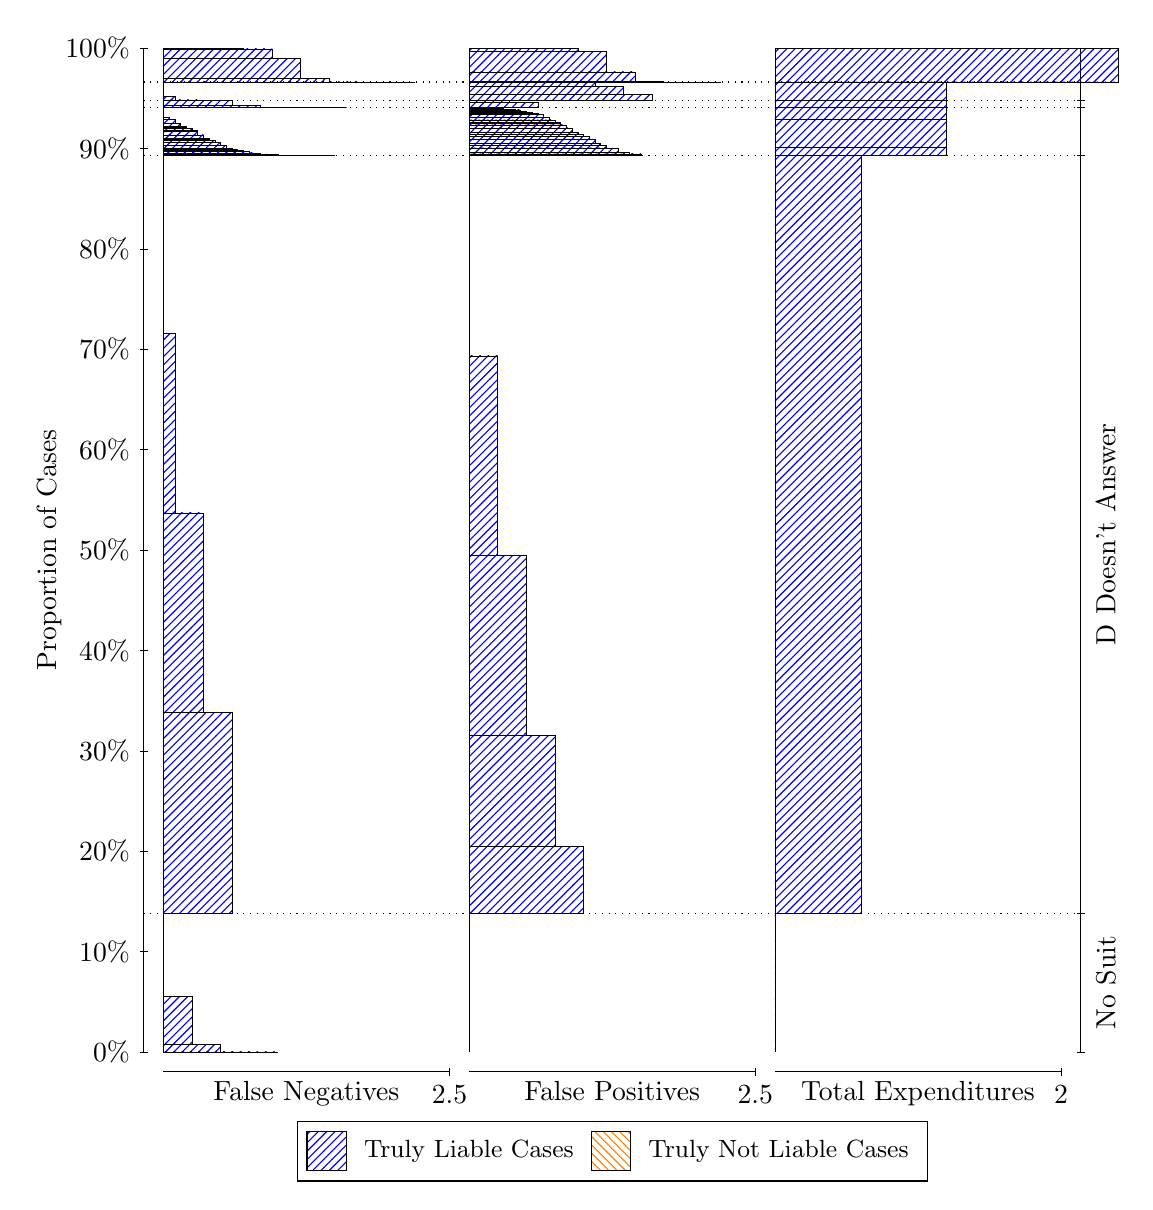
\begin{tikzpicture}
\draw[black, very thin] (1.5,1.75) -- (1.5,14.5);
\node[rotate=90, text=black, anchor=center] at (0.3, 8.125) {Proportion of Cases};
\draw[black, very thin] (1.45,1.75) -- (1.55,1.75);
\node[text=black, anchor=east] at (1.45, 1.75) {0\%};
\draw[black, very thin] (1.45,3.025) -- (1.55,3.025);
\node[text=black, anchor=east] at (1.45, 3.025) {10\%};
\draw[black, very thin] (1.45,4.3) -- (1.55,4.3);
\node[text=black, anchor=east] at (1.45, 4.3) {20\%};
\draw[black, very thin] (1.45,5.575) -- (1.55,5.575);
\node[text=black, anchor=east] at (1.45, 5.575) {30\%};
\draw[black, very thin] (1.45,6.85) -- (1.55,6.85);
\node[text=black, anchor=east] at (1.45, 6.85) {40\%};
\draw[black, very thin] (1.45,8.125) -- (1.55,8.125);
\node[text=black, anchor=east] at (1.45, 8.125) {50\%};
\draw[black, very thin] (1.45,9.4) -- (1.55,9.4);
\node[text=black, anchor=east] at (1.45, 9.4) {60\%};
\draw[black, very thin] (1.45,10.675) -- (1.55,10.675);
\node[text=black, anchor=east] at (1.45, 10.675) {70\%};
\draw[black, very thin] (1.45,11.95) -- (1.55,11.95);
\node[text=black, anchor=east] at (1.45, 11.95) {80\%};
\draw[black, very thin] (1.45,13.225) -- (1.55,13.225);
\node[text=black, anchor=east] at (1.45, 13.225) {90\%};
\draw[black, very thin] (1.45,14.5) -- (1.55,14.5);
\node[text=black, anchor=east] at (1.45, 14.5) {100\%};

\draw[black, very thin] (13.4,1.75) -- (13.4,14.5);
\draw[black, very thin] (13.35,1.75) -- (13.45,1.75);
\node[anchor=west] at (13.35, 1.75) {};
\draw[black, very thin] (13.35,3.512) -- (13.45,3.512);
\node[anchor=west] at (13.35, 3.512) {};
\draw[black, very thin] (13.35,13.139) -- (13.45,13.139);
\node[anchor=west] at (13.35, 13.139) {};
\draw[black, very thin] (13.35,13.744) -- (13.45,13.744);
\node[anchor=west] at (13.35, 13.744) {};
\draw[black, very thin] (13.35,13.835) -- (13.45,13.835);
\node[anchor=west] at (13.35, 13.835) {};
\draw[black, very thin] (13.35,14.068) -- (13.45,14.068);
\node[anchor=west] at (13.35, 14.068) {};
\draw[black, very thin] (13.35,14.5) -- (13.45,14.5);
\node[anchor=west] at (13.35, 14.5) {};

\draw[black, very thin, pattern color=blue, pattern=north east lines] (1.75,1.75) rectangle (3.2033,1.75);
\draw[black, very thin, pattern color=blue, pattern=north east lines] (1.75,1.75) rectangle (2.84,1.7508);
\draw[black, very thin, pattern color=blue, pattern=north east lines] (1.75,1.7508) rectangle (2.4767,1.8508);
\draw[black, very thin, pattern color=blue, pattern=north east lines] (1.75,1.8508) rectangle (2.1133,2.46);
\draw[black, very thin, pattern color=orange, pattern=north west lines] (1.75,2.46) rectangle (1.75,2.46);
\draw[black, very thin, pattern color=blue, pattern=north east lines] (1.75,2.46) rectangle (1.75,3.512);
\draw[black, very thin, pattern color=blue, pattern=north east lines] (1.75,3.512) rectangle (2.622,6.0618);
\draw[black, very thin, pattern color=blue, pattern=north east lines] (1.75,6.0618) rectangle (2.2587,8.5964);
\draw[black, very thin, pattern color=blue, pattern=north east lines] (1.75,8.5964) rectangle (1.8953,10.879);
\draw[black, very thin, pattern color=orange, pattern=north west lines] (1.75,10.879) rectangle (1.75,10.879);
\draw[black, very thin, pattern color=blue, pattern=north east lines] (1.75,10.879) rectangle (1.75,13.139);
\draw[black, very thin, pattern color=blue, pattern=north east lines] (1.75,13.139) rectangle (3.93,13.139);
\draw[black, very thin, pattern color=blue, pattern=north east lines] (1.75,13.139) rectangle (3.7847,13.139);
\draw[black, very thin, pattern color=blue, pattern=north east lines] (1.75,13.139) rectangle (3.6393,13.139);
\draw[black, very thin, pattern color=blue, pattern=north east lines] (1.75,13.139) rectangle (3.5667,13.139);
\draw[black, very thin, pattern color=blue, pattern=north east lines] (1.75,13.139) rectangle (3.494,13.139);
\draw[black, very thin, pattern color=blue, pattern=north east lines] (1.75,13.139) rectangle (3.4213,13.139);
\draw[black, very thin, pattern color=blue, pattern=north east lines] (1.75,13.139) rectangle (3.3487,13.139);
\draw[black, very thin, pattern color=blue, pattern=north east lines] (1.75,13.139) rectangle (3.276,13.139);
\draw[black, very thin, pattern color=blue, pattern=north east lines] (1.75,13.139) rectangle (3.2033,13.149);
\draw[black, very thin, pattern color=blue, pattern=north east lines] (1.75,13.149) rectangle (3.1307,13.15);
\draw[black, very thin, pattern color=blue, pattern=north east lines] (1.75,13.15) rectangle (3.058,13.15);
\draw[black, very thin, pattern color=blue, pattern=north east lines] (1.75,13.15) rectangle (3.058,13.157);
\draw[black, very thin, pattern color=blue, pattern=north east lines] (1.75,13.157) rectangle (2.9853,13.158);
\draw[black, very thin, pattern color=blue, pattern=north east lines] (1.75,13.158) rectangle (2.9127,13.168);
\draw[black, very thin, pattern color=blue, pattern=north east lines] (1.75,13.168) rectangle (2.9127,13.168);
\draw[black, very thin, pattern color=blue, pattern=north east lines] (1.75,13.168) rectangle (2.84,13.188);
\draw[black, very thin, pattern color=blue, pattern=north east lines] (1.75,13.188) rectangle (2.7673,13.196);
\draw[black, very thin, pattern color=blue, pattern=north east lines] (1.75,13.196) rectangle (2.6947,13.198);
\draw[black, very thin, pattern color=blue, pattern=north east lines] (1.75,13.198) rectangle (2.6947,13.215);
\draw[black, very thin, pattern color=blue, pattern=north east lines] (1.75,13.215) rectangle (2.622,13.226);
\draw[black, very thin, pattern color=blue, pattern=north east lines] (1.75,13.226) rectangle (2.5493,13.266);
\draw[black, very thin, pattern color=blue, pattern=north east lines] (1.75,13.266) rectangle (2.5493,13.267);
\draw[black, very thin, pattern color=blue, pattern=north east lines] (1.75,13.267) rectangle (2.4767,13.297);
\draw[black, very thin, pattern color=blue, pattern=north east lines] (1.75,13.297) rectangle (2.404,13.306);
\draw[black, very thin, pattern color=blue, pattern=north east lines] (1.75,13.306) rectangle (2.404,13.324);
\draw[black, very thin, pattern color=blue, pattern=north east lines] (1.75,13.324) rectangle (2.3313,13.336);
\draw[black, very thin, pattern color=blue, pattern=north east lines] (1.75,13.336) rectangle (2.3313,13.357);
\draw[black, very thin, pattern color=blue, pattern=north east lines] (1.75,13.357) rectangle (2.2587,13.397);
\draw[black, very thin, pattern color=blue, pattern=north east lines] (1.75,13.397) rectangle (2.186,13.44);
\draw[black, very thin, pattern color=blue, pattern=north east lines] (1.75,13.44) rectangle (2.186,13.45);
\draw[black, very thin, pattern color=blue, pattern=north east lines] (1.75,13.45) rectangle (2.1133,13.48);
\draw[black, very thin, pattern color=blue, pattern=north east lines] (1.75,13.48) rectangle (2.0407,13.49);
\draw[black, very thin, pattern color=blue, pattern=north east lines] (1.75,13.49) rectangle (2.0407,13.509);
\draw[black, very thin, pattern color=blue, pattern=north east lines] (1.75,13.509) rectangle (1.968,13.547);
\draw[black, very thin, pattern color=blue, pattern=north east lines] (1.75,13.547) rectangle (1.8953,13.591);
\draw[black, very thin, pattern color=blue, pattern=north east lines] (1.75,13.591) rectangle (1.8227,13.615);
\draw[black, very thin, pattern color=orange, pattern=north west lines] (1.75,13.615) rectangle (1.75,13.615);
\draw[black, very thin, pattern color=blue, pattern=north east lines] (1.75,13.615) rectangle (1.75,13.744);
\draw[black, very thin, pattern color=blue, pattern=north east lines] (1.75,13.744) rectangle (4.0753,13.744);
\draw[black, very thin, pattern color=blue, pattern=north east lines] (1.75,13.744) rectangle (3.712,13.744);
\draw[black, very thin, pattern color=blue, pattern=north east lines] (1.75,13.744) rectangle (3.3487,13.746);
\draw[black, very thin, pattern color=blue, pattern=north east lines] (1.75,13.746) rectangle (2.9853,13.771);
\draw[black, very thin, pattern color=blue, pattern=north east lines] (1.75,13.771) rectangle (2.622,13.835);
\draw[black, very thin, pattern color=orange, pattern=north west lines] (1.75,13.835) rectangle (1.75,13.835);
\draw[black, very thin, pattern color=blue, pattern=north east lines] (1.75,13.835) rectangle (2.622,13.835);
\draw[black, very thin, pattern color=blue, pattern=north east lines] (1.75,13.835) rectangle (2.2587,13.842);
\draw[black, very thin, pattern color=blue, pattern=north east lines] (1.75,13.842) rectangle (1.8953,13.886);
\draw[black, very thin, pattern color=orange, pattern=north west lines] (1.75,13.886) rectangle (1.75,13.886);
\draw[black, very thin, pattern color=blue, pattern=north east lines] (1.75,13.886) rectangle (1.75,14.068);
\draw[black, very thin, pattern color=blue, pattern=north east lines] (1.75,14.068) rectangle (4.9473,14.068);
\draw[black, very thin, pattern color=blue, pattern=north east lines] (1.75,14.068) rectangle (4.584,14.068);
\draw[black, very thin, pattern color=blue, pattern=north east lines] (1.75,14.068) rectangle (4.2207,14.069);
\draw[black, very thin, pattern color=blue, pattern=north east lines] (1.75,14.069) rectangle (3.8573,14.115);
\draw[black, very thin, pattern color=blue, pattern=north east lines] (1.75,14.115) rectangle (3.494,14.37);
\draw[black, very thin, pattern color=blue, pattern=north east lines] (1.75,14.37) rectangle (3.1307,14.488);
\draw[black, very thin, pattern color=blue, pattern=north east lines] (1.75,14.488) rectangle (2.7673,14.5);
\draw[black, very thin, pattern color=blue, pattern=north east lines] (1.75,14.5) rectangle (2.404,14.5);
\draw[black, very thin, pattern color=blue, pattern=north east lines] (1.75,14.5) rectangle (2.0407,14.5);
\draw[black, very thin, pattern color=orange, pattern=north west lines] (1.75,14.5) rectangle (1.75,14.5);
\draw[black, very thin, pattern color=orange, pattern=north west lines] (5.6333,1.75) rectangle (5.6333,1.75);
\draw[black, very thin, pattern color=blue, pattern=north east lines] (5.6333,1.75) rectangle (5.6333,3.512);
\draw[black, very thin, pattern color=orange, pattern=north west lines] (5.6333,3.512) rectangle (7.0867,3.512);
\draw[black, very thin, pattern color=blue, pattern=north east lines] (5.6333,3.512) rectangle (7.0867,4.359);
\draw[black, very thin, pattern color=blue, pattern=north east lines] (5.6333,4.359) rectangle (6.7233,5.771);
\draw[black, very thin, pattern color=blue, pattern=north east lines] (5.6333,5.771) rectangle (6.36,8.0541);
\draw[black, very thin, pattern color=blue, pattern=north east lines] (5.6333,8.0541) rectangle (5.9967,10.589);
\draw[black, very thin, pattern color=blue, pattern=north east lines] (5.6333,10.589) rectangle (5.6333,13.139);
\draw[black, very thin, pattern color=orange, pattern=north west lines] (5.6333,13.139) rectangle (7.8133,13.139);
\draw[black, very thin, pattern color=blue, pattern=north east lines] (5.6333,13.139) rectangle (7.8133,13.155);
\draw[black, very thin, pattern color=orange, pattern=north west lines] (5.6333,13.155) rectangle (7.668,13.155);
\draw[black, very thin, pattern color=blue, pattern=north east lines] (5.6333,13.155) rectangle (7.668,13.178);
\draw[black, very thin, pattern color=orange, pattern=north west lines] (5.6333,13.178) rectangle (7.5227,13.178);
\draw[black, very thin, pattern color=blue, pattern=north east lines] (5.6333,13.178) rectangle (7.5227,13.222);
\draw[black, very thin, pattern color=blue, pattern=north east lines] (5.6333,13.222) rectangle (7.45,13.233);
\draw[black, very thin, pattern color=orange, pattern=north west lines] (5.6333,13.233) rectangle (7.3773,13.233);
\draw[black, very thin, pattern color=blue, pattern=north east lines] (5.6333,13.233) rectangle (7.3773,13.268);
\draw[black, very thin, pattern color=blue, pattern=north east lines] (5.6333,13.268) rectangle (7.3047,13.292);
\draw[black, very thin, pattern color=orange, pattern=north west lines] (5.6333,13.292) rectangle (7.232,13.292);
\draw[black, very thin, pattern color=blue, pattern=north east lines] (5.6333,13.292) rectangle (7.232,13.335);
\draw[black, very thin, pattern color=blue, pattern=north east lines] (5.6333,13.335) rectangle (7.1593,13.373);
\draw[black, very thin, pattern color=orange, pattern=north west lines] (5.6333,13.373) rectangle (7.0867,13.373);
\draw[black, very thin, pattern color=blue, pattern=north east lines] (5.6333,13.373) rectangle (7.0867,13.402);
\draw[black, very thin, pattern color=blue, pattern=north east lines] (5.6333,13.402) rectangle (7.014,13.433);
\draw[black, very thin, pattern color=orange, pattern=north west lines] (5.6333,13.433) rectangle (6.9413,13.433);
\draw[black, very thin, pattern color=blue, pattern=north east lines] (5.6333,13.433) rectangle (6.9413,13.485);
\draw[black, very thin, pattern color=blue, pattern=north east lines] (5.6333,13.485) rectangle (6.8687,13.525);
\draw[black, very thin, pattern color=orange, pattern=north west lines] (5.6333,13.525) rectangle (6.796,13.525);
\draw[black, very thin, pattern color=blue, pattern=north east lines] (5.6333,13.525) rectangle (6.796,13.546);
\draw[black, very thin, pattern color=blue, pattern=north east lines] (5.6333,13.546) rectangle (6.796,13.559);
\draw[black, very thin, pattern color=blue, pattern=north east lines] (5.6333,13.559) rectangle (6.7233,13.586);
\draw[black, very thin, pattern color=orange, pattern=north west lines] (5.6333,13.586) rectangle (6.6507,13.586);
\draw[black, very thin, pattern color=blue, pattern=north east lines] (5.6333,13.586) rectangle (6.6507,13.615);
\draw[black, very thin, pattern color=blue, pattern=north east lines] (5.6333,13.615) rectangle (6.578,13.657);
\draw[black, very thin, pattern color=blue, pattern=north east lines] (5.6333,13.657) rectangle (6.5053,13.668);
\draw[black, very thin, pattern color=blue, pattern=north east lines] (5.6333,13.668) rectangle (6.4327,13.685);
\draw[black, very thin, pattern color=blue, pattern=north east lines] (5.6333,13.685) rectangle (6.4327,13.686);
\draw[black, very thin, pattern color=blue, pattern=north east lines] (5.6333,13.686) rectangle (6.36,13.695);
\draw[black, very thin, pattern color=blue, pattern=north east lines] (5.6333,13.695) rectangle (6.2873,13.715);
\draw[black, very thin, pattern color=blue, pattern=north east lines] (5.6333,13.715) rectangle (6.2147,13.725);
\draw[black, very thin, pattern color=blue, pattern=north east lines] (5.6333,13.725) rectangle (6.142,13.725);
\draw[black, very thin, pattern color=blue, pattern=north east lines] (5.6333,13.725) rectangle (6.0693,13.733);
\draw[black, very thin, pattern color=blue, pattern=north east lines] (5.6333,13.733) rectangle (6.0693,13.733);
\draw[black, very thin, pattern color=blue, pattern=north east lines] (5.6333,13.733) rectangle (5.9967,13.733);
\draw[black, very thin, pattern color=blue, pattern=north east lines] (5.6333,13.733) rectangle (5.924,13.744);
\draw[black, very thin, pattern color=blue, pattern=north east lines] (5.6333,13.744) rectangle (5.8513,13.744);
\draw[black, very thin, pattern color=blue, pattern=north east lines] (5.6333,13.744) rectangle (5.7787,13.744);
\draw[black, very thin, pattern color=blue, pattern=north east lines] (5.6333,13.744) rectangle (5.706,13.744);
\draw[black, very thin, pattern color=blue, pattern=north east lines] (5.6333,13.744) rectangle (5.6333,13.744);
\draw[black, very thin, pattern color=orange, pattern=north west lines] (5.6333,13.744) rectangle (6.5053,13.744);
\draw[black, very thin, pattern color=blue, pattern=north east lines] (5.6333,13.744) rectangle (6.5053,13.808);
\draw[black, very thin, pattern color=blue, pattern=north east lines] (5.6333,13.808) rectangle (6.142,13.833);
\draw[black, very thin, pattern color=blue, pattern=north east lines] (5.6333,13.833) rectangle (5.7787,13.835);
\draw[black, very thin, pattern color=blue, pattern=north east lines] (5.6333,13.835) rectangle (5.6333,13.835);
\draw[black, very thin, pattern color=orange, pattern=north west lines] (5.6333,13.835) rectangle (7.9587,13.835);
\draw[black, very thin, pattern color=blue, pattern=north east lines] (5.6333,13.835) rectangle (7.9587,13.915);
\draw[black, very thin, pattern color=blue, pattern=north east lines] (5.6333,13.915) rectangle (7.5953,14.017);
\draw[black, very thin, pattern color=blue, pattern=north east lines] (5.6333,14.017) rectangle (7.232,14.061);
\draw[black, very thin, pattern color=blue, pattern=north east lines] (5.6333,14.061) rectangle (6.8687,14.068);
\draw[black, very thin, pattern color=blue, pattern=north east lines] (5.6333,14.068) rectangle (6.5053,14.068);
\draw[black, very thin, pattern color=orange, pattern=north west lines] (5.6333,14.068) rectangle (8.8307,14.068);
\draw[black, very thin, pattern color=blue, pattern=north east lines] (5.6333,14.068) rectangle (8.8307,14.068);
\draw[black, very thin, pattern color=blue, pattern=north east lines] (5.6333,14.068) rectangle (8.4673,14.068);
\draw[black, very thin, pattern color=orange, pattern=north west lines] (5.6333,14.068) rectangle (8.4673,14.068);
\draw[black, very thin, pattern color=blue, pattern=north east lines] (5.6333,14.068) rectangle (8.4673,14.068);
\draw[black, very thin, pattern color=blue, pattern=north east lines] (5.6333,14.068) rectangle (8.104,14.069);
\draw[black, very thin, pattern color=orange, pattern=north west lines] (5.6333,14.069) rectangle (8.104,14.069);
\draw[black, very thin, pattern color=blue, pattern=north east lines] (5.6333,14.069) rectangle (8.104,14.08);
\draw[black, very thin, pattern color=blue, pattern=north east lines] (5.6333,14.08) rectangle (7.7407,14.08);
\draw[black, very thin, pattern color=orange, pattern=north west lines] (5.6333,14.08) rectangle (7.7407,14.08);
\draw[black, very thin, pattern color=blue, pattern=north east lines] (5.6333,14.08) rectangle (7.7407,14.198);
\draw[black, very thin, pattern color=blue, pattern=north east lines] (5.6333,14.198) rectangle (7.3773,14.198);
\draw[black, very thin, pattern color=orange, pattern=north west lines] (5.6333,14.198) rectangle (7.3773,14.198);
\draw[black, very thin, pattern color=blue, pattern=north east lines] (5.6333,14.198) rectangle (7.3773,14.453);
\draw[black, very thin, pattern color=blue, pattern=north east lines] (5.6333,14.453) rectangle (7.014,14.499);
\draw[black, very thin, pattern color=blue, pattern=north east lines] (5.6333,14.499) rectangle (6.6507,14.5);
\draw[black, very thin, pattern color=blue, pattern=north east lines] (5.6333,14.5) rectangle (6.2873,14.5);
\draw[black, very thin, pattern color=blue, pattern=north east lines] (5.6333,14.5) rectangle (5.924,14.5);
\draw[black, very thin, pattern color=orange, pattern=north west lines] (9.5167,1.75) rectangle (9.5167,1.75);
\draw[black, very thin, pattern color=blue, pattern=north east lines] (9.5167,1.75) rectangle (9.5167,3.512);
\draw[black, very thin, pattern color=orange, pattern=north west lines] (9.5167,3.512) rectangle (10.607,3.512);
\draw[black, very thin, pattern color=blue, pattern=north east lines] (9.5167,3.512) rectangle (10.607,13.139);
\draw[black, very thin, pattern color=orange, pattern=north west lines] (9.5167,13.139) rectangle (11.697,13.139);
\draw[black, very thin, pattern color=blue, pattern=north east lines] (9.5167,13.139) rectangle (11.697,13.234);
\draw[black, very thin, pattern color=orange, pattern=north west lines] (9.5167,13.234) rectangle (11.697,13.234);
\draw[black, very thin, pattern color=blue, pattern=north east lines] (9.5167,13.234) rectangle (11.697,13.59);
\draw[black, very thin, pattern color=orange, pattern=north west lines] (9.5167,13.59) rectangle (11.697,13.59);
\draw[black, very thin, pattern color=blue, pattern=north east lines] (9.5167,13.59) rectangle (11.697,13.744);
\draw[black, very thin, pattern color=orange, pattern=north west lines] (9.5167,13.744) rectangle (11.697,13.744);
\draw[black, very thin, pattern color=blue, pattern=north east lines] (9.5167,13.744) rectangle (11.697,13.835);
\draw[black, very thin, pattern color=orange, pattern=north west lines] (9.5167,13.835) rectangle (11.697,13.835);
\draw[black, very thin, pattern color=blue, pattern=north east lines] (9.5167,13.835) rectangle (11.697,14.068);
\draw[black, very thin, pattern color=orange, pattern=north west lines] (9.5167,14.068) rectangle (13.877,14.068);
\draw[black, very thin, pattern color=blue, pattern=north east lines] (9.5167,14.068) rectangle (13.877,14.07);
\draw[black, very thin, pattern color=orange, pattern=north west lines] (9.5167,14.07) rectangle (13.877,14.07);
\draw[black, very thin, pattern color=blue, pattern=north east lines] (9.5167,14.07) rectangle (13.877,14.5);
\draw[black, dotted] (1.5,3.512) -- (13.4,3.512);
\draw[black, dotted] (1.5,13.139) -- (13.4,13.139);
\draw[black, dotted] (1.5,13.744) -- (13.4,13.744);
\draw[black, dotted] (1.5,13.835) -- (13.4,13.835);
\draw[black, dotted] (1.5,14.068) -- (13.4,14.068);
\draw[black, very thin] (1.75,1.5) -- (5.3833,1.5);
\node[text=black, anchor=north] at (3.5667, 1.5) {False Negatives};
\draw[black, very thin] (5.3833,1.45) -- (5.3833,1.55);
\node[text=black, anchor=north] at (5.3833, 1.45) {2.5};

\draw[black, very thin] (5.6333,1.5) -- (9.2667,1.5);
\node[text=black, anchor=north] at (7.45, 1.5) {False Positives};
\draw[black, very thin] (9.2667,1.45) -- (9.2667,1.55);
\node[text=black, anchor=north] at (9.2667, 1.45) {2.5};

\draw[black, very thin] (9.5167,1.5) -- (13.15,1.5);
\node[text=black, anchor=north] at (11.333, 1.5) {Total Expenditures};
\draw[black, very thin] (13.15,1.45) -- (13.15,1.55);
\node[text=black, anchor=north] at (13.15, 1.45) {2};

\node[text=black, centered, rotate=90] at (13.72, 2.631) {No Suit};
\node[text=black, centered, rotate=90] at (13.72, 8.3253) {D Doesn't Answer};





\draw (7.449999999999999,1.5) node[draw=none] (baseCoordinate) {};
\begin{scope}[align=center]
        \matrix[scale=0.5, draw=black, below=0.5cm of baseCoordinate, nodes={draw}, column sep=0.1cm]{
            \node[rectangle, draw, minimum width=0.5cm, minimum height=0.5cm, pattern color=blue, pattern=north east lines] {}; &
            \node[draw=none, font=\small, text=black] (B) {Truly Liable Cases}; &
            \node[rectangle, draw, minimum width=0.5cm, minimum height=0.5cm, pattern color=orange, pattern=north west lines] {}; &
            \node[draw=none, font=\small, text=black] (B) {Truly Not Liable Cases}; \\
            };
\end{scope}

\end{tikzpicture}
\end{document}